\documentclass[11pt]{article}

\usepackage[margin=1in]{geometry}
\usepackage{booktabs}
\usepackage{hyperref}
\usepackage{amsmath}
\usepackage{graphicx}
\usepackage{url}
\usepackage{tikz}
\usepackage{placeins}
\usepackage{xcolor}
\usetikzlibrary{arrows.meta,positioning,shapes.geometric}

\title{TestGate: Why Evidence Beats Uncertainty for Local LLM Reliability}
\author{Rana Muhammad Usman\\
\texttt{usmanashrafrana@gmail.com}}
\date{February 2026}

\begin{document}
\maketitle

\begin{abstract}
Local language models offer privacy and low cost but frequently produce unreliable outputs---
malformed JSON, failing code, or invalid SQL. We present \textbf{TestGate}, an open-source
toolkit providing three reliability strategies as separate modes: (1) \textit{uncertainty-based
routing} using token-level entropy and margin from logprobs, (2) \textit{evidence-gated routing}
using test execution to decide escalation, and (3) \textit{contract-first generation} using
JSON schema validation with repair loops.

We evaluate these strategies on HumanEval (code) and structured output tasks (JSON, SQL).
Our key finding is counter-intuitive: \textbf{uncertainty-based routing hurts code generation}
(pass@1 drops from 0.54 to 0.42), while \textbf{evidence-gated routing helps significantly}
(pass@1 improves from 0.54 to 0.72, beating even the larger model alone at 0.68). For structured outputs, contract-first generation improves validity
dramatically for code-specialized models (0.70 to 1.00) but can hurt general-purpose models.

We provide practical guidelines: use evidence-gating when tests exist, contract-first for
structured output with code-specialized models, and avoid uncertainty-based routing for code.
TestGate is released as open-source to help practitioners build reliable local LLM applications.
\end{abstract}

\section{Introduction}

Local LLMs are increasingly deployed for privacy-sensitive and cost-conscious applications.
However, reliability remains a critical barrier: models produce syntactically invalid outputs,
code that fails tests, or structured data that doesn't match schemas. Unlike hosted APIs with
guaranteed structured output modes, local deployments must handle reliability at the application layer.

We address a practical question: \textbf{How should local LLM applications detect and recover
from unreliable outputs?} Prior work has explored constrained decoding~\cite{outlines,guidance},
API-level structured outputs~\cite{openai_structured_outputs}, and prompt engineering. We take
a different approach: \textit{post-generation reliability strategies} that work with any local
model without modifying the inference engine.

We present \textbf{TestGate}, a toolkit with three strategies:

\begin{enumerate}
\item \textbf{Uncertainty-based routing}: Use token-level logprobs to estimate confidence.
      Escalate to a larger model or repair uncertain spans when entropy is high or margin is low.

\item \textbf{Evidence-gated routing}: For tasks with verifiable outputs (code with tests),
      run the output and only escalate if it fails. This uses ground truth rather than proxy signals.

\item \textbf{Contract-first generation}: Request structured JSON matching a schema, validate,
      repair if invalid, then compile to final artifacts (SQL, code stubs).
\end{enumerate}

Our empirical evaluation yields surprising findings. On HumanEval code generation:
\begin{itemize}
\item Uncertainty-based escalation \textit{reduces} pass@1 from 0.54 to 0.52
\item Uncertainty-based repair \textit{reduces} pass@1 from 0.54 to 0.42
\item Evidence-gated routing \textit{improves} pass@1 from 0.54 to 0.72 (+18 percentage points)
\end{itemize}

On structured output tasks:
\begin{itemize}
\item Contract-first improves SQL validity from 0.00 to 1.00 (code-specialized models)
\item Contract-first \textit{reduces} validity from 0.96 to 0.68 (general-purpose models)
\end{itemize}

These results challenge common assumptions and provide actionable guidelines for practitioners.
We release TestGate as open-source at \url{https://github.com/ranausmanai/testgate}.

\section{Related Work}

\textbf{Constrained decoding.}
Outlines~\cite{outlines} uses finite-state machines to guarantee outputs match JSON schemas.
Guidance~\cite{guidance} interleaves generation with programmatic constraints.
SGLang~\cite{sglang} compiles structured programs into efficient execution plans.
LMQL~\cite{lmql} provides a query language for constrained LLM generation.
Grammar-based sampling in llama.cpp~\cite{llamacpp_grammar} restricts tokens via BNF grammars.
These require inference engine integration, which may not be available for all deployments.

\textbf{Uncertainty estimation in LLMs.}
Token-level entropy and probability margins have been used for selective prediction~\cite{selective_prediction}
and calibration. Speculative decoding~\cite{speculative_decoding} uses small models to draft
tokens verified by larger models. Our uncertainty-based routing extends these ideas to
full-output escalation and repair.

\textbf{Test-driven code generation.}
Self-repair approaches~\cite{self_repair} use test feedback to iteratively fix code.
CodeT~\cite{codet} generates tests alongside code for self-consistency.
Our evidence-gating is simpler: run once, escalate on failure, no iteration.

\textbf{Structured output validation.}
Instructor~\cite{instructor} validates against Pydantic schemas with retry.
Jsonformer~\cite{jsonformer} guarantees JSON structure by generating only variable portions.
Our contract-first approach adds compilation to executable artifacts (SQL, code).

\section{The TestGate Toolkit}

TestGate provides three reliability strategies as separate CLI modes. Each mode takes a prompt
and model configuration, returning output along with metadata about the strategy applied.

\begin{figure}[h]
\centering
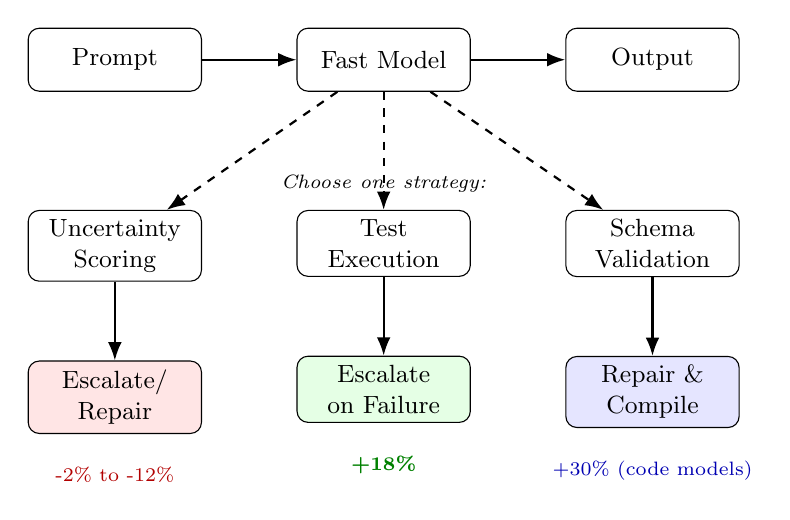
\begin{tikzpicture}[
    node distance=1cm and 1.2cm,
    box/.style={draw, rounded corners, align=center, minimum width=2.2cm, minimum height=0.8cm, font=\small},
    arrow/.style={-Latex, thick}
]
% Top row
\node[box] (input) {Prompt};
\node[box, right=of input] (fast) {Fast Model};
\node[box, right=of fast] (output) {Output};

% Three strategy paths (below)
\node[box, below=1.5cm of input] (s1) {Uncertainty\\Scoring};
\node[box, below=1.5cm of fast] (s2) {Test\\Execution};
\node[box, below=1.5cm of output] (s3) {Schema\\Validation};

% Actions
\node[box, below=of s1, fill=red!10] (a1) {Escalate/\\Repair};
\node[box, below=of s2, fill=green!10] (a2) {Escalate\\on Failure};
\node[box, below=of s3, fill=blue!10] (a3) {Repair \&\\Compile};

% Result labels
\node[below=0.3cm of a1, font=\scriptsize, text=red!70!black] {-2\% to -12\%};
\node[below=0.3cm of a2, font=\scriptsize, text=green!50!black] {\textbf{+18\%}};
\node[below=0.3cm of a3, font=\scriptsize, text=blue!70!black] {+30\% (code models)};

% Main flow arrows
\draw[arrow] (input) -- (fast);
\draw[arrow] (fast) -- (output);

% Strategy arrows
\draw[arrow, dashed] (fast) -- (s1);
\draw[arrow, dashed] (fast) -- (s2);
\draw[arrow, dashed] (fast) -- (s3);

\draw[arrow] (s1) -- (a1);
\draw[arrow] (s2) -- (a2);
\draw[arrow] (s3) -- (a3);

% Labels
\node[above=0.1cm of s2, font=\scriptsize\itshape] {Choose one strategy:};
\end{tikzpicture}
\caption{Three reliability strategies with their impact on output quality. Evidence-gating (center) provides the largest improvement for code generation.}
\label{fig:framework}
\end{figure}

\subsection{Strategy 1: Uncertainty-Based Routing}

We compute per-token uncertainty from logprobs provided by the model backend.

\textbf{Entropy.} For each token, we compute entropy over the top-$k$ logprobs:
\[
H_i = -\sum_{j=1}^{k} p_{ij} \log p_{ij}
\]
where $p_{ij}$ is the normalized probability of the $j$-th most likely token at position $i$.

\textbf{Margin.} The probability gap between the top two tokens:
\[
M_i = p_{i1} - p_{i2}
\]

A token is flagged as \textit{uncertain} if $H_i > \tau_H$ or $M_i < \tau_M$ (defaults: $\tau_H=0.65$, $\tau_M=0.08$).
If more than $N$ tokens are uncertain (default: 4), we trigger escalation or repair.

\textbf{Escalation.} Re-generate with a larger/slower model, optionally passing the draft as context.

\textbf{Selective Repair.} Instead of full re-generation, identify uncertain spans and ask the
model to produce targeted JSON patches:
\begin{verbatim}
{"edits": [{"before": "...", "after": "..."}]}
\end{verbatim}
This preserves correct portions of the output while fixing uncertain regions.

\subsection{Strategy 2: Evidence-Gated Routing}

For tasks with verifiable outputs (code with test cases), we use execution feedback instead of
uncertainty estimates.

\begin{enumerate}
\item Generate output with the fast model
\item Execute tests on the output
\item If tests pass: return output (no escalation needed)
\item If tests fail: escalate to slow model with error feedback
\end{enumerate}

This approach has a key advantage: it uses \textit{ground truth} rather than proxy signals.
A model may be confident but wrong, or uncertain but correct. Tests resolve this ambiguity.

\subsection{Strategy 3: Contract-First Generation}

For structured outputs (JSON, SQL, code stubs), we decompose generation into steps:

\begin{enumerate}
\item \textbf{Contract prompt}: Request JSON matching a strict schema
\item \textbf{Validation}: Parse and validate against the schema
\item \textbf{Repair}: If invalid, request correction (with error message)
\item \textbf{Compilation}: Deterministically compile JSON to final artifact
\end{enumerate}

For SQL, the contract is a JSON AST:
\begin{verbatim}
{"select": ["col1", "col2"], "from": "users",
 "where": [{"col": "age", "op": ">", "val": 18}],
 "order_by": [{"col": "name", "dir": "ASC"}]}
\end{verbatim}
which compiles to: \texttt{SELECT col1, col2 FROM users WHERE age > 18 ORDER BY name ASC}

This moves syntactic correctness from the model to the compiler.

\section{Experimental Setup}

\subsection{Tasks and Benchmarks}

\textbf{Code generation.} HumanEval~\cite{humaneval}, subset of 50 tasks (the first 50 by task ID).
We measure pass@1 with execution-based evaluation. All results are from runs archived in the
repository under \texttt{eval/runs/}.

\textbf{Structured output.} Custom benchmark with 50 prompts: 20 JSON extraction,
15 SQL generation, 15 Python code stubs. We measure syntactic validity.

\subsection{Models}

All experiments use local models via Ollama:
\begin{itemize}
\item \textbf{Fast}: qwen2.5-coder:7b (code-specialized)
\item \textbf{Slow}: qwen2.5-coder:14b (code-specialized, larger)
\item \textbf{General}: llama3.2:3b (general-purpose)
\end{itemize}

\subsection{Configurations}

\textbf{Uncertainty routing}: entropy threshold 0.65, margin threshold 0.08, min uncertain tokens 4-10.

\textbf{Evidence-gating}: 5-second timeout per test execution.

\textbf{Contract-first}: 1 repair attempt, temperature 0.0.

All experiments run on consumer hardware (Apple M4, 24GB RAM).

\textbf{Reproducibility.} All runs use the same 50 HumanEval tasks (IDs 0--49 plus 100--113).
Artifacts are archived in the repository: 7B baseline and evidence-gating from
\texttt{eval/runs/unified-paper/}, 14B baseline from \texttt{eval/runs/baseline-14b/},
uncertainty routing from \texttt{eval/runs/20260205-162415/}.

\section{Results}

\subsection{Code Generation (HumanEval)}

\begin{table}[h]
\centering
\begin{tabular}{lrrrr}
\toprule
Strategy & Pass@1 & Gen Time (s) & Slow Used & Change \\
\midrule
Baseline (7b only) & 0.54 & 543 & 0\% & --- \\
Baseline (14b only) & 0.68 & 669 & 100\% & +14\% \\
Uncertainty $\rightarrow$ Escalate & 0.52 & 874 & 36\% & \textcolor{red}{-2\%} \\
Uncertainty $\rightarrow$ Repair & 0.42 & 943 & n/a & \textcolor{red}{-12\%} \\
\midrule
Evidence-Gating (7b$\rightarrow$14b) & \textbf{0.72} & 1109 & 46\% & \textcolor{green}{+18\%} \\
\bottomrule
\end{tabular}
\caption{HumanEval results. Uncertainty-based routing hurts; evidence-gating helps.}
\label{tab:humaneval}
\end{table}

\textbf{Key finding}: Uncertainty-based routing \textit{degrades} code generation quality.
The model often produces high-entropy outputs that are actually correct, or low-entropy
outputs that are wrong. Logprob uncertainty is not a reliable signal for code correctness.

Evidence-gating shows the opposite pattern: by using actual test execution, we escalate
only when tests fail (46\% of tasks), and the slow model successfully fixes 9 of those 23 failures,
boosting pass@1 from 0.54 to 0.72.

\subsection{Structured Output}

\begin{table}[h]
\centering
\begin{tabular}{llrrrr}
\toprule
Model & Strategy & Valid Rate & Avg Sec & Repair Rate & Change \\
\midrule
Qwen 7B & Baseline & 0.70 & 4.7 & 0\% & --- \\
Qwen 7B & Contract & \textbf{1.00} & 8.0 & 6\% & \textcolor{green}{+30\%} \\
\midrule
Llama 3B & Baseline & 0.96 & 3.4 & 0\% & --- \\
Llama 3B & Contract & 0.68 & 12.4 & 36\% & \textcolor{red}{-28\%} \\
\bottomrule
\end{tabular}
\caption{Structured output results. Contract-first helps code-specialized models, hurts general models.}
\label{tab:structured}
\end{table}

\textbf{Key finding}: Contract-first generation is highly effective for code-specialized models
but counterproductive for general-purpose models. The SQL contract format (JSON AST) is
natural for models trained on code; general models struggle with the added structure.

\subsection{Per-Task Analysis}

\begin{table}[h]
\centering
\begin{tabular}{llrr}
\toprule
Task Type & Model & Baseline & Contract \\
\midrule
JSON & Qwen 7B & 1.00 & 1.00 \\
JSON & Llama 3B & 1.00 & 1.00 \\
\midrule
SQL & Qwen 7B & 0.00 & \textbf{1.00} \\
SQL & Llama 3B & 1.00 & 0.20 \\
\midrule
Code Stub & Qwen 7B & 1.00 & 1.00 \\
Code Stub & Llama 3B & 0.87 & 0.73 \\
\bottomrule
\end{tabular}
\caption{Validity by task type. SQL shows the most dramatic model-dependent behavior.}
\label{tab:bytask}
\end{table}

SQL generation shows the starkest contrast: Qwen's baseline produces 0\% valid SQL (format
confusion, prose mixed with queries), while contract-first achieves 100\%. Llama's baseline
produces valid SQL directly, but the contract format confuses it.

\section{Analysis and Discussion}

\subsection{Why Does Uncertainty Routing Fail for Code?}

We analyzed cases where uncertainty routing made wrong decisions:

\textbf{False positives}: Correct code flagged as uncertain. The model may use rare but
valid syntax (list comprehensions, lambda expressions) that have high entropy but are correct.

\textbf{False negatives}: Incorrect code with low uncertainty. The model confidently produces
plausible-looking code with subtle bugs (off-by-one errors, wrong variable names).

Code correctness is \textit{semantic}, not syntactic. Uncertainty measures syntactic confidence,
which is orthogonal to whether the code actually works.

\subsection{Why Does Evidence-Gating Work?}

Evidence-gating uses the only reliable signal for code: execution. This has limitations
(requires tests, only catches failures that tests cover) but avoids the false positive/negative
problem entirely.

The pass@1 gain is substantial: 54\% to 72\% (+18 points). Of 50 tasks, 27 passed immediately
on the fast model, and of the 23 that failed and escalated, the slow model fixed 9.
Crucially, evidence-gating (72\%) even beats using the 14b model alone (68\%), while using
the slow model for only 46\% of tasks. This shows the value of selective escalation:
the fast model's correct outputs are preserved, while failures get a second chance.

\subsection{Why Does Contract-First Depend on Model Type?}

Code-specialized models (Qwen-Coder) are trained on structured formats: JSON, SQL, code.
The contract format aligns with their training distribution.

General-purpose models (Llama) may not have seen SQL AST formats. The contract adds cognitive
load, leading to more errors than direct SQL generation.

\textbf{Implication}: Match the reliability strategy to the model's strengths.

\section{Practical Guidelines}

Based on our findings, we recommend:

\begin{table}[h]
\centering
\begin{tabular}{llll}
\toprule
Task & Tests Available? & Model Type & Recommended Strategy \\
\midrule
Code & Yes & Any & \textbf{Evidence-gating} \\
Code & No & Any & Baseline (no reliable signal) \\
\midrule
SQL/JSON & No & Code-specialized & \textbf{Contract-first} \\
SQL/JSON & No & General & Baseline only \\
\bottomrule
\end{tabular}
\caption{Decision matrix for choosing reliability strategies.}
\label{tab:guidelines}
\end{table}

\textbf{Do not} use uncertainty-based routing for code generation---it hurts more than it helps.

\textbf{Do} use evidence-gating when tests exist; the overhead is minimal and the gains are real.

\textbf{Do} use contract-first for structured output, but only with code-specialized models.

\section{Limitations}

\textbf{Benchmark scale.} HumanEval has 164 problems; we evaluated 50. Structured output uses
a custom 50-prompt benchmark. Larger-scale evaluation would strengthen claims.

\textbf{Model coverage.} We tested two model families (Qwen, Llama). Results may differ for
other architectures (Mistral, Phi, etc.).

\textbf{Evidence-gating scope.} Requires test cases, which don't exist for all code tasks.
Not applicable to non-code domains without oracles.

\textbf{Uncertainty thresholds.} We used default thresholds; task-specific tuning might help.
However, the fundamental issue (semantic vs. syntactic confidence) likely remains.

\section{Conclusion}

We presented TestGate, a toolkit for improving local LLM reliability through adaptive
strategies. Our key contributions:

\begin{enumerate}
\item \textbf{Counter-intuitive finding}: Uncertainty-based routing hurts code generation.
      Models are often confident when wrong and uncertain when correct.

\item \textbf{Evidence-gating works}: Using test execution as the escalation signal improves
      pass@1 by 18 percentage points (0.54 to 0.72), escalating only on observed test failure.

\item \textbf{Model-dependent strategies}: Contract-first generation helps code-specialized
      models dramatically but hurts general-purpose models.

\item \textbf{Practical guidelines}: A decision matrix for choosing strategies based on
      task type, test availability, and model characteristics.
\end{enumerate}

TestGate is released as open-source to help practitioners build reliable local LLM
applications. We hope these findings save others from the common assumption that
``more uncertainty = escalate'' is always beneficial.

\bibliographystyle{plain}
\bibliography{references_unified}

\end{document}
